\addbibresource{mybib.bib}
\section{A function prediction method}
\subsection*{Prologue}
As we mentioned in the introduction our main goal was to develop a
a classification algorithm for the PLC probelm which can be used for the
purpose of protein function prediction in a partially annotated PPI
network.

What it means is we are going to take an input a strongly connected
graph where the vertices represent protein types and the edges represent
observed interaction between them. The some of the proteins are
annotated with a label that specifies their function. The rest are
unannotated.

The prediction algorithm is going to output for each unlabeled protein a
proposed label. Our paradigm is that protein is that proteins of the
same label should form, approximately, a community in the sennse of
graph community structure which we discussed in the earlier sections.
Since the algorithm is using propagation methods which are closely
related to the community structure of the graph, if the paradigm doesn't
hold then the prediction sohould be no better than a coin toss.

It is understood that proteins that interact are more likely than not to
share the same function~\cite{schwikowski2000network}. It's a weaker
property than our paradigm because it doesn't speak about communities,
only about adjacent proteins.

The diffusion matrix provides us with ranking such that for for every
vertex $i$ we can weigh the other vertices by 'importance' to that
vertice (namely it's the $i$ row of the diffusion matrix). We use that
information to predict the label of the protein. We assume that members
of the same label of the protein will have cummulatively the most
'influence' on it. We also assume that the distribution of labeled and
unlabeled is the same across the network so by removing them from
consideration, still the proteins that share the same label with the
protein we test will have the most cummulative influence on it.

\subsection*{}

Section 4 gave us a strong indication about the usefulness of the
diffusion matrix as as a type of quasi-distance with which we
measure closeness or 'influence' between nodes in the network.
Our working paradigm is that connected nodes are more likely to have
the same functional class than not, a fact which has been shown to
be true by \textcite{schwikowski2000network}.

In this section we are going to apply the accumulated knowledge of the
previous sections and devise some simple function prediction algorithms for PPI
networks. We to try several methods which use propagation as well as
methods which just use direct neighbors for the predictions.

The network is going to be composed of around 500 vertices (proteins) which are
divided into 4 different function groups. We are going to randomly choose half
the proteins and mark them as unknown and try to predict their function based
on the remaining known proteins. Then we can verify the results with the
actual annotations.

\subsection{Tools and Source Data}

We sourced our data from \textcite{cytoscape}, an open source
java software for network analysis and visualisation. 
The software as one of its built in examples a
fully annotated yeast interactome. This is a PPI network of
thousands of proteins and it contains among many other types of
edge and node annotations information about protein function and
location in the 'MCs name' field.

We preferred to work within the familiar Python 3 programming
language and its rich world of extension libraries and packages.
Therefore we exported the yeast interactome into a graphml format
which was later imported into our network analysis tool of choice,
\textcite{networkx}. This is a python based open sourced network analysis 
package which integrates extremely well with other essential Python
packages. Networkx is neither as versatile nor as powerful as Cytoscape and
especially rudimentary in its visualisation functionality, but it
runs smoothly and is easy to work with, unlike Cytoscape.
We used the \textcite{numpy} package for vector, matrix and other
types mathematical
calculations, and \textcite{pandas} for some database operations. 

\subsection{Methodology}
As mentioned, we 
used the annotated yeast interactome which is a pure PPI network that comes
prepackaged with the
software tool 'Cytoscape'. The nodes represent yeast proteins and the edges
represent protein-protein interactions.

This network comes with functional annotations in the 'MCs name' field.
We selected nodes in the network whose annotations contain
\textbf{exactly} one of the following keywords:  'DNA Replication' (blue
group), 'Golgi' (red), 'Meiosis' (yellow), and 'Stress response'
(green). All other nodes are removed from the network.  The result is
shown in figure \ref{fig:yeast_subgraph_4groups}.

The resulting subnetwork is not a connected graph, which is the type
of input data that we wanted to run our test algorithm on. Therefore
we selected the biggest connected component of that subnetwork, and
that is the graph on which we tested and compared various prediction
algorithms.

\begin{figure}
\begin{framed}
\centering
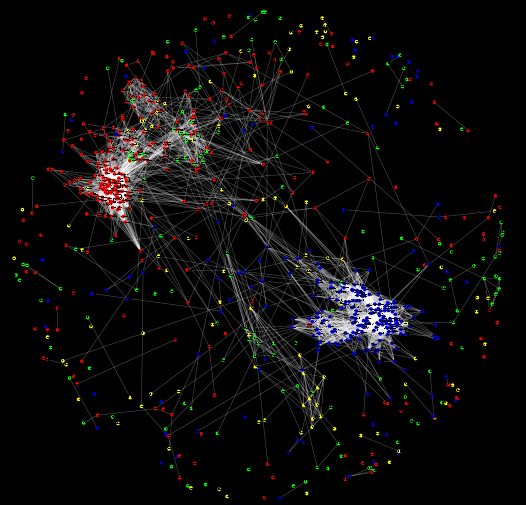
\includegraphics[width=\textwidth]{figures/yeastsubgraph_4_groups_colorcode.png}
\caption{Subgraph of the yeast interactome showing nodes of 4 groups: 'DNA
replication' (blue), 'Golgi' (red), 'Meiosis' (yellow), 'Stress response'
(green)}
\label{fig:yeast_subgraph_4groups}
\end{framed}
\end{figure}

For the first set of comparative tests of different prediction
methods 
we set a random seed (a process which we repeat 2 times for 2 different trials).
Then we selected randomly 50\% of the nodes and marked them as 'unknown'. The other
50\% are 'known'. We would then try to determine the group affiliation of the
unknown nodes based on the group affiliations of the known nodes.

We tried 5 different prediction methods:

\begin{itemize}
\item{Method 1} Determines the group affiliation of an unknown node by the group
that has the maximal volume based on the propagation distribution from the
unknown node. This meas: we calculate the stationary distribution with restart
to the unknown node. Among the known nodes, we calculate the weighted sums of
each of the 4 groups according to that distribution. The group with largest
volume is the affiliation we assign to the unknown node.

\item{Method 2} This method works like method 1, except that we first order the
unknown nodes (decreasing order) according to their pageRank. We go over the
nodes in this order and assign group affiliation according to method 1, but then
we also update the list of the known nodes to include that node. So this node is
going to be included in the function prediction of the lower ranked nodes.

The rational here is that the higher ranked nodes are probably going to be
predicted with high accuracy and therefore be helpful in prediction of lower
ranked nodes. 

It is probably better to device some simple rule to decide whether it is worth
to include a node in the prediction of the rest of the nodes. For example, based
on how many unknown neighbors in has vs known neighbors. But we tried to keep
things simple at this stage.

\item{Method 3} We assign an unknown node to the group that has plurality among
its neighbors with known group affiliation. So this method is fast and
probably the simplest.

\item{Method 4} Same as method 3, but again we go in the order of pagRanks and
we update the list of known nodes on the fly, like method 2.

\item{Method 5} Here we take each group of the known nodes and propagate from
it. So for example we calculate the stationary distribution when we restart in
the known nodes that belong to group 'DNA Replication', and then for the next
group and so forth. For each unknown node, we assign it to the group that
propagates the highest probability to it.

While in method 1 and 2 we start random walking from an unknown node and see
what is the probability that we land at a certain group, In Method 5 we start
walking randomly from one of the members of a group and check what is the
probability that we visit a certain unknown node.

This method is an order of magnitude faster than method 1 and 2 because we only
need to calculate the stationary distributions 4 time (pageRank and for each
group). However we suspect it will perform with less accuracy.
The reason for that is that method 5 takes into account nodes that are far and not well connected to the
unknown node whose function we try to predict.
The function groups, in particular the yellow (meiosis) and green (stress) are not
well clustered and spread all over the network but we can see that
some subsets of these labels form clusters.

\end{itemize}

\subsection{Some code snippets}
\begin{lstlisting}[language=python]
# The decision function which is used in methods 1 and 2 to predict a single
# node
# This version uses a stored diffusion kernel to calculate the
# propagation, rather than using the power method multiple times.
def decision_function_diffkernel(v, G, K, group_membership_ar, known_unknown_ar):
    """
    This function uses the given diffusion kernel of the graph to
    calculate the propagation, rather than using the power method.
    Input v: an node assumed to be an int and taken from the list of unkown
    nodes. Input G: The graph.
    Input K: the diffusion kernel of the graph.
    Input group_membership_ar: Array of strings which specifies for each node
    to which group belongs (including the 'unkonw' nodes) this is required for
    thesting the correctness of the decision.
    Input known_unknown_ar: boolean 1d array which
    specifies for each node of the graph whether its membership is known or
    unkown.
    output prediction: A string which is the predicted group affiliation.
    output correctness: True or false depending on the correctness of the
    prediction vs the real group_membership_list[v] value.
    """
    all_nodes = np.arange(len(G.nodes))
    known_nodes = all_nodes[known_unknown_ar]
    unknown_nodes = all_nodes[known_unknown_ar == False]
    bias = np.zeros_like(G.nodes)
    bias[v] = 1
    bias
    p = np.dot(K, bias)
    group_names = np.unique(group_membership_ar)
    q = p * known_unknown_ar  # 0 on all unkown nodes
    testscores = np.zeros_like(group_names)
    for g in range(len(group_names)):
        x = q[group_membership_ar == group_names[g]]
        testscores[g] = x.sum()
    decide = group_names[np.argmax(testscores)]
    correctness = decide == group_membership_ar[v]
    return decide, correctness

def predictMethod2_diffkernel(G, tries=1, knownfraction=0.5, seed=42, alpha=0.2):
    """
    Like predictMethod2 but uses diffusion kernel rather than power
    method.
    Input G: a graph.
    Input tries: how many repetitions to perform, each witha
    different randomly selected 'known' group.
    Input knownfraction: portion of the known nodes out all the
    nodes.
    Input seed: random seed.
    Input alpha: restart parameter.
    """
    groups = [G.nodes[x]["Group"] for x in G.nodes()]
    groups = np.array(groups)  # array is better than a simple list ...
    group_labeling = np.unique(groups)
    df = pd.DataFrame()
    df["Group (ground truth)"] = groups
    scores = np.zeros(tries)
    # determine the pageRanks
    K = diffKernelG(G, alpha=alpha)
    pageRank = biasedPropagateGA(G, bias=np.ones_like(G.nodes), alpha=0.2)
    orderedNodeList = np.argsort(pageRank)
    # set the random seed
    np.random.seed(seed=seed)
    for t in range(tries):
        groups_predict = groups.copy()
        known_unknown = np.random.random(len(G.nodes)) < knownfraction  # known=1
        all_nodes = np.arange(len(G.nodes))
        known_nodes = all_nodes[known_unknown]
        unknown_nodes = all_nodes[known_unknown == False]
        orderedUnkownNodeList = orderedNodeList[known_unknown == False]
        known_unknown2 = known_unknown.copy()
        score2 = 0
        df["Rep " + str(t)] = "known"
        df["Rep " + str(t) + "_predict"] = groups_predict
        for v in orderedUnkownNodeList:
            # predict, test = decision_function(v, G, groups, known_unknown2, alpha=alpha)
            #predict, test = decision_function_diffkernel(
            #    v, G, K, groups, known_unknown2
            #)
            predict, test = decision_function_diffkernel(
                v, G, K, groups_predict, known_unknown2
            )
            groups_predict[v] = predict
            score2 += test
            known_unknown2[v] = True  # mark v as 'known'
            df["Rep " + str(t)][v] = "correct"
            df["Rep " + str(t) + "_predict"][v] = predict
            if not test:  # mark as incorrect and colormark if mistake
                df["Rep " + str(t)][v] = "mistake"
        score2 = score2 / len(unknown_nodes)  # got 0.85
        scores[t] = score2
    return scores, df
\end{lstlisting}

\subsection{Results}

\begin{table}[!htb]
\caption{Prediction Accuracy of the 4 Methods in 2 different random
trials. Each trial with a different seed, which result in different randomly
selected known/unknown nodes.} 
\begin{center}
\begin{tabular}{ | l | c | c | c | c | c | }
\hline
Seed / Method & 1 & 2 & 3 & 4 & 5\\
\hline
42 & 0.795 & 0.854 & 0.765 &
0.791 & 0.701\\
6382020 & 0.774 & 0.832 & 0.751 & 0.751 & 0.755\\
\hline
\end{tabular}
\label{table:results_5_prediction_methods}
\end{center}
\end{table}

We decided to further experiment with method 2.
We tested it with different parameters, repeating each settings 50 times
with 50 different sets of known labels. The parameters we tested were
the restart probability ($\alpha$) and what we called the labeled
coverage, which is the portion of the nodes that start with a known
label.
The best mean result (for coverage of 0.5), was $0.8926$ mean accuracy.
It was obtained with a
restart probability of $0.31$. Restart parameters $\alpha \in [0.2-0.3]5$, lets
call it mid-lower range, produce the best results, while with higher
alphas accuracy falls towards $0.5$ which is of course the accuracy of
just randomly guessing. 

Accuracy was about 0.8 when we start with only 10\% labeled and it
gradually increases with increased labeled proportions (0.85 accuracy at
0.3 label coverage). We plotted the relationship between accuracy and
the parameters in figure \ref{fig:alpha_fracs}.

\begin{figure}
\begin{framed}
\centering
\begin{subfigure}[b]{\textwidth}
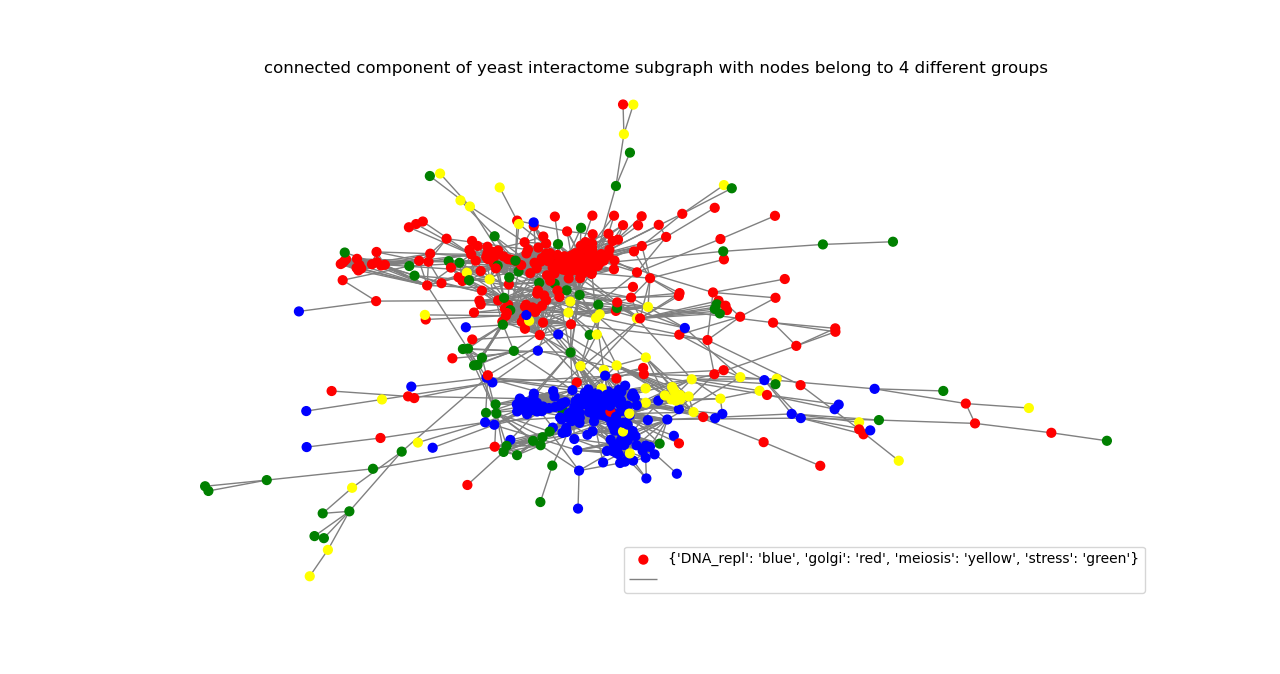
\includegraphics[width=\textwidth]{figures/connected component of yeast interactome subgraph with nodes belong to 4 different groups.png}
\caption{The largest connected component which was selected for the function
prediction experiment. Here the Correct group affiliation of all nodes is color
coded.}
\label{fig:largest_connected_comp}
\end{subfigure}
\begin{subfigure}[b]{\textwidth}
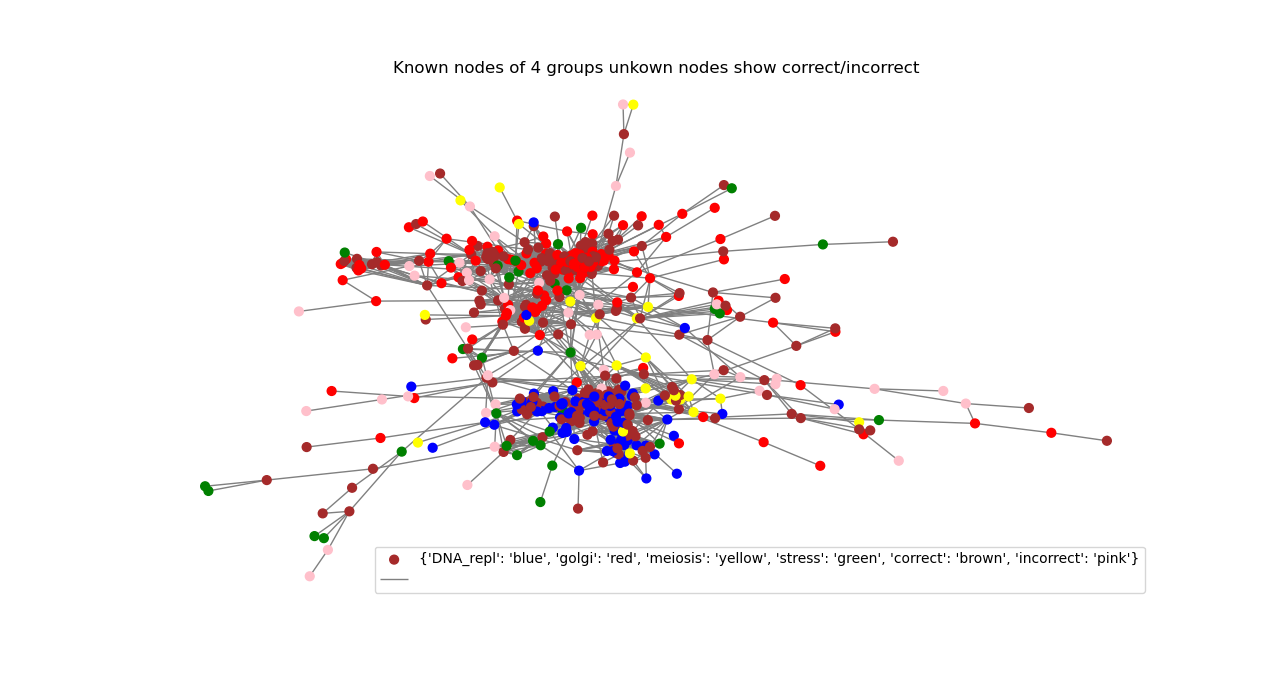
\includegraphics[width=\textwidth]{figures/method2_true_false_clustering_on_4_groups_with_ordering_and_update.png}
\caption{The result of predictiob method 2, which was the best perfomer. 
The known groups are color coded by RGBY. The unkown nodes are color
coded: brown:correct prediction, pink:incorrect.}
\label{fig:my_prediction}
\end{subfigure}
\end{framed}
\end{figure}

We have conducted another test of method 2, with parameters $\alpha =
0.31$, and label coverage of $0.35$.
This time we calculated the sensitivity, specificity, accuracy and
precision (PPV) 
for each label as well as the total.
The results are the following:
\begin{lstlisting}[basicstyle=\footnotesize]
      Label      P     TP    FP        N       TN    FN Sens Spec  Acc  PPV
0     golgi    165    149    25      209      184    16 0.90 0.88 0.89 0.86
1  DNA_repl    133    129    22      241      219     4 0.97 0.91 0.93 0.85
2   meiosis     30     17     4      344      340    13 0.57 0.99 0.95 0.81
3    stress     46     25     3      328      325    21 0.54 0.99 0.94 0.89
4     Total 374.00 320.00 54.00 1,122.00 1,068.00 54.00 0.86 0.95 0.93 0.86
\end{lstlisting}
\label{tab:senspec}

We can see that the problem lies with the two small and spread out groups,
'meiosis' and 'stress'. It is hard to predict that an unlabeled vertex belong to these groups 

\begin{figure}
\begin{framed}
\centering
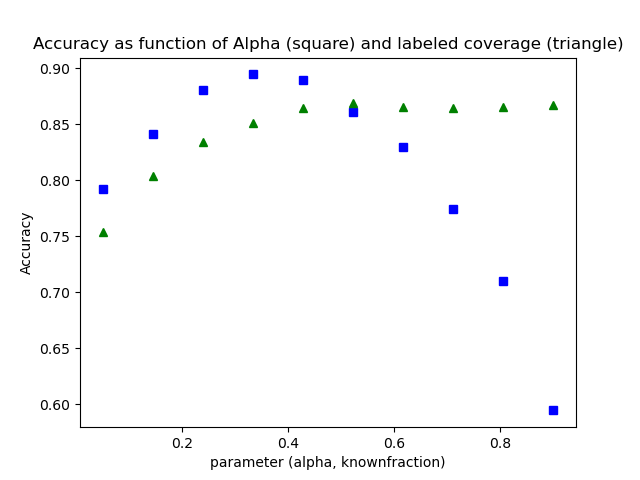
\includegraphics[width=\textwidth]{figures/alpha_fraq_graph.png}
\caption{The accuracy as function of the resart parameter alpha,
with fixed label coverage of 0.5, and of the label coverage with
fixed alpha=0.2}
\label{fig:alpha_fracs}
\end{framed}
\end{figure}

\subsection{Discussion}
If we look at figure \ref{fig:largest_connected_comp} which shows the connected
component that we worked with, the red and blue are pretty nicely clustered. The
greens and specially the yellows are sort of spread all over the network and
not nicely clustered. I don't know if this is a good example of a real world
scenario.

When we look at figure \ref{fig:my_prediction} it seems that most of the
incorrect predictions are on nodes that seem 'peripheral' and  are not well
connected to known nodes. Another source of mistakes seems to bee green nodes
that are too close to the red cluster.

Method 2 shows somewhat higher accuracy over the other methods but on the flip
side it is an $O(n^2)$ method when optimized methods are used whereas methods
3,4,5 are $O(n)$.
